\documentclass[10pt,twocolumn,letterpaper]{article}

\usepackage{cvpr}
\usepackage{times}
\usepackage{epsfig}
\usepackage{graphicx}
\usepackage{amsmath}
\usepackage{amssymb}
\usepackage{eso-pic}  %Required
\usepackage{helvet}  %Required
\usepackage{courier}  %Required
\usepackage{url}  %Required
\usepackage{graphicx}  %Required
\frenchspacing  %Required
\usepackage{mathrsfs}
% \usepackage{color}
\usepackage{multirow}
% \usepackage{subfigure}
% \usepackage{comment}
% \usepackage{mathrsfs}
% \usepackage{lipsum}
\usepackage{bbm}
\usepackage{enumerate}

\usepackage{xcolor}
\usepackage{soul}
\usepackage[utf8]{inputenc}
\usepackage[small]{caption}

\usepackage{booktabs}       % professional-quality tables
\usepackage{amsfonts}       % blackboard math symbols
\usepackage{nicefrac}       % compact symbols for 1/2, etc.
\usepackage{microtype}      % microtypography
\usepackage{bbm}
\usepackage{subfigure}
\usepackage{comment}
\usepackage[numbers]{natbib}

% Include other packages here, before hyperref.

% If you comment hyperref and then uncomment it, you should delete
% egpaper.aux before re-running latex.  (Or just hit 'q' on the first latex
% run, let it finish, and you should be clear).
\usepackage[pagebackref=true,breaklinks=true,letterpaper=true,colorlinks,bookmarks=false]{hyperref}

% \cvprfinalcopy % *** Uncomment this line for the final submission

\def\cvprPaperID{****} % *** Enter the CVPR Paper ID here
\def\httilde{\mbox{\tt\raisebox{-.5ex}{\symbol{126}}}}

% Pages are numbered in submission mode, and unnumbered in camera-ready
\ifcvprfinal\pagestyle{empty}\fi
\begin{document}

%%%%%%%%% TITLE
\title{Memory In Memory: Differential Recurrent Neural Networks for\\ Spatiotemporal Prediction}

\author{First Author\\
Institution1\\
Institution1 address\\
{\tt\small firstauthor@i1.org}
% For a paper whose authors are all at the same institution,
% omit the following lines up until the closing ``}''.
% Additional authors and addresses can be added with ``\and'',
% just like the second author.
% To save space, use either the email address or home page, not both
\and
Second Author\\
Institution2\\
First line of institution2 address\\
{\tt\small secondauthor@i2.org}
}

\maketitle
%\thispagestyle{empty}

%%%%%%%%% ABSTRACT
\begin{abstract}
   A spatiotemporal predictive model aims to generate future frames by observing existing context, in which stationarity and non-stationarity are two significant features. Most previous work based on recurrent networks, with relatively simple memory transition functions over time, mainly focus on the stationary component. However, it proves difficult for these models to handle the more complicated non-stationary variations. In this paper, we present a differential recurrent neural network named Memory In Memory (MIM). The core of our model is the MIM block that takes in the differential features between adjacent recurrent states, and models the spatiotemporal stationary and non-stationary patterns separately. It uses two self-renewed memory units to handle these two components. The MIM model achieves the state-of-the-art results on three spatiotemporal prediction datasets, including a synthetic dataset and two real datasets, and is believed to be a potentially generic architecture for time-series modeling.
\end{abstract}

%%%%%%%%% BODY TEXT
\section{Introduction}
\label{sec:Introduction}
In recent years, spatiotemporal predictive learning techniques have made great improvements in real applications, including traffic flows prediction \citep{zhang2017deep} and precipitation forecasting \citep{shi2015convolutional,wang2017predrnn}. A well-performed predictive learning system is expected to learn the intrinsic variations in the consecutive spatiotemporal context, which can be seen as a combination of two components: the stationary and the non-stationary. 

A great challenge in spatiotemporal prediction is that most existing work, including the ConvLSTM network \citep{shi2015convolutional} and PredRNN \citep{wang2017predrnn}, focuses on stationary variations with simple transition functions between the recurrent states. This leads to a phenomenon that the predicted frames generated by these models become increasingly blurred over time. It is possibly caused by the inconsistency between the non-stationary spatiotemporal dynamics and an approximately linear extrapolation system.

Although in these LSTM \citep{hochreiter1997long} based models, recurrent gate structures (especially the forget gate) are used to deliver, select, and discard information in the memory states temporal transitions paths. These gate structures are a little bit simple for capturing the complicated and non-stationary variations in the high-dimensional spatiotemporal data. In our preliminary experiments, we find that the forget gates in the PredRNN model \citep{wang2017predrnn} do not work in an appropriate way. For most of time, over 80 percent of them are saturated, implying that this model always remembers similar variations. In another word, what is learned is mainly the stationary component. 

Inspired by this observation, we focus on a more appropriate memory transition function for spatiotemporal modeling. We assume that this transition function is a combination of the stationary and non-stationary variations, and treat them separately in a more explicit way. It is simpler to capture the stationary variations, such as a fixed speed of a moving object. It can be seemed as the very short-term trends in spatiotemporal data. The non-stationary component, such as the noise, the sudden changes, or the unexpected occlusions of multiple moving objects, evolves over time and is more complicated to capture. It could be partially tackled by solving the long-term reasoning problem. But there is still a long way towards spatiotemporal reasoning. 

Our idea is more straightforward. Noting that the differential features are widely exploited in non-deep autoregressive models for non-stationary dynamics \citep{percival1993spectral} while not fully exploited in deep networks, we propose a new recurrent block named Memory In Memory (MIM) to leverage the differential information between adjacent recurrent states. Inside the MIM block, we inject a second-order recurrent module to replace the original recurrent memory transitions. 
This module has two inner recurrent units respectively for capturing the non-stationary variations from the differential features, and the stationary variations. In LSTM terms, this module can be seen as an improved version of forget gate that models the memory state transitions. But in fact, it is no longer a standard gate structure. Instead, the two inner units hold their own memory cells and are self-renewed over time, as the outer memory cell in the MIM does. This mechanism is therefore intuitively named ``memory in memory''. The proposed Differential Recurrent Neural Network (DRNN) achieves the state-of-the-art results on three video spatiotemporal prediction datasets, including a synthetic dataset, a real human activity dataset, and a real traffic flows dataset.

\section{Related Work}
\label{sec:Related}
In recent years, deep learning has made breakthroughs in several areas. Many great work based on convolutional neural network \citep{krizhevsky2012imagenet} and recurrent neural network \citep{Sutskever2014Sequence} provides a lot of useful insights for spatiotemporal prediction. Inspired by language modeling, Ranzato \textit{et al.} \citep{Ranzato2014Video} defined a RNN architecture predicting frames in a discrete space of patch clusters. Srivastava \textit{et al.} \citep{srivastava2015unsupervised} defined a sequence to sequence LSTM framework for video prediction. But this sequence to sequence model can only capture temporal dependencies. Shi \textit{et al.} \citep{shi2015convolutional} combined RNN and CNN by proposing a convolutional LSTM network, which learns spatial and temporal dependencies simultaneously. %But these convolutional recurrent models took a lot of time and memory space in the training process. 
Finn \textit{et al.} \citep{Finn2016Unsupervised} developed an action-conditioned video prediction model that predicts a distribution over pixel motion from previous frames. Villegas \textit{et al.} \citep{Villegas2017Decomposing} also built a model upon ConvLSTMs with optical flow guided features. Patraucean \textit{et al.} \citep{patraucean2015spatio} defined a model that generates optical flow frames for every input frame, then applies the optical flow frame to the current frame to generate the next frame. Kalchbrenner \textit{et al.} \citep{Kalchbrenner2016Video} proposed the Video Pixel Network (VPN) that encodes the time, space and color structures of video tensors as a four-dimensional dependency chain. This model uses the well-established PixelCNNs \citep{van2016conditional}, and achieves sharp prediction results. However it suffers from a high computational complexity. Wang \textit{et al.} \citep{wang2017predrnn} presented a spatiotemporal LSTM unit with dual memory structures. This structure has a zigzag memory flow and provides a great modeling capability of short-term modeling. %\citet{Oh2015Action} proposed two autoencoder neural network architectures based on CNN and RNN, and used it to predict frames in Atari games. 
Mathieu \textit{et al.} \citep{Mathieu2015Deep} defined a CNN-based model using generative adversarial networks (GAN) \citep{Goodfellow2014Generative,Denton2015Deep}. Vondrick \textit{et al.} \citep{vondrick2016generating} also used adversarial learning to generate frames from noise vectors by applying it on 3D CNNs. 

More recently, there have been some methods that aim to model the stochasticity in spatiotemporal predictive learning. %\citep{fraccaro2016sequentia}
These methods argue that future uncertainty is the cause of the blurry predictions. Henceforth, Variational Autoencoder (VAE) \citep{kingma2013auto} is introduced to spatiotemporal predictive learning to generate stochastic latent variables and use them as a component in the prediction making process. Lee \textit{et al.} \citep{lee2018stochastic} designed a similar approach to explicitly model the stochasticity in future predictions and combined it with the adversarial training method. Denton \textit{et al.} \citep{denton2018stochastic} proposed another VAE based video prediction model that learns a prior of uncertainty in a given environment. These methods increase the diversity of the prediction results, but are difficult to evaluate and required to run a great number of times. In this paper, we focus on the deterministic part of spatiotemporal predictive learning, divide it into stationary and non-stationary modeling, and attempt to capture complex data variations in the historical observations.

%% PredRNN: temporal dynamics

%In this paper, we present a new spatiotemporal recurrent block and make contributions in two aspects: (1) A new sequence to sequence model with oblique information flow is designed to exploit the differential information from spatiotemporal data. (2) Use two cascaded recurrent memory units to handle stationary and non-stationary variations respectively.

%------------------------------------------------------------------------
\section{Preliminaries}
\label{sec:Preliminaries}
PredRNN \citep{wang2017predrnn} has made a remarkable improvement in video prediction. It allows the memory states and hidden states to be delivered in two directions: across cascaded RNN layers vertically and through all RNN states horizontally. This mechanism is implemented by the spatiotemporal LSTM (ST-LSTM) units, which almost double the gate structures in traditional convolutional LSTMs \citep{shi2015convolutional}. Via these gates, the output states of a certain ST-LSTM unit are determined by the spatiotemporal memory $\mathcal{M}_t^{l-1}$ passed from the previous layer, as well as the temporal memory $\mathcal{C}_{t-1}^l$ delivered from the previous time stamp. Calculations inside a spatiotemporal LSTM unit at time stamp $t$ and layer $l$ are shown as follows:
\begin{equation}\label{equ:stlstm}
  \small
  \begin{split}
  & g_t = \tanh(W_{xg} \ast \mathcal{X}_t + W_{hg} \ast \mathcal{H}_{t-1}^l + b_g) \\
  & i_t = \sigma(W_{xi} \ast \mathcal{X}_t + W_{hi} \ast \mathcal{H}_{t-1}^l + b_i) \\
  & f_t = \sigma(W_{xf} \ast \mathcal{X}_t + W_{hf} \ast \mathcal{H}_{t-1}^l + b_f) \\
  & \mathcal{C}_t^l = f_t \odot \mathcal{C}_{t-1}^l + i_t \odot g_t \\
  & g_t^\prime = \tanh(W_{xg}^\prime \ast \mathcal{X}_t + W_{mg} \ast \mathcal{M}_t^{l-1} + b_g^\prime) \\
  & i_t^\prime = \sigma(W_{xi}^\prime \ast \mathcal{X}_t + W_{mi} \ast \mathcal{M}_t^{l-1} + b_i^\prime) \\
  & f_t^\prime = \sigma(W_{xf}^\prime \ast \mathcal{X}_t + W_{mf} \ast \mathcal{M}_t^{l-1} + b_f^\prime) \\
  & \mathcal{M}_t^l = f_t^\prime \odot \mathcal{M}_t^{l-1} + i_t^\prime \odot g_t^\prime \\
  & o_t = \sigma(W_{xo} \ast \mathcal{X}_t + W_{ho} \ast \mathcal{H}_{t-1}^l + W_{co} \ast \mathcal{C}_t^l + W_{mo} \ast \mathcal{M}_t^l + b_o) \\ 
  & \mathcal{H}_t^l = o_t \odot \tanh(W_{1\times1} \ast [\mathcal{C}_t^l, \mathcal{M}_t^l]),\\
  \end{split}
\end{equation}
where $\sigma$ is the sigmoid activation function, $\ast$ and $\odot$ denote the convolution and the Hadamard product operators respectively. The input gate $i_t$, input modulation gate $g_t$, forget gate $f_t$ and output gate $o_t$ control spatiotemporal information flows. The unit at time stamp $t$ and layer $l$ has four inputs: $\mathcal{X}_t$, which is either the input frame for $l=1$ or the output hidden states by the previous layer $\mathcal{H}_t^{l-1}$ for $l>1$; $\mathcal{H}_{t-1}^l$ and $\mathcal{C}_{t-1}^l$, the hidden states and memory states from the previous time stamp; as well as $\mathcal{M}_t^{l-1}$, the spatiotemporal memory states either from the top layer at the previous time stamp or the last layer at the current time stamp. All states are represented by $\mathbb{R}^{C \times W \times H}$ dimensional tensors, where the first dimension is the number of their channels, and the following two dimensions denote the height and width of feature maps. The structure of ST-LSTM is shown in Figure \ref{fig:node} (left).

The biggest highlight of PredRNN is its zigzag memory flow of the spatiotemporal memory $\mathcal{M}$. It provides PredRNN a great modeling capability of the short-term trends in longer pathways through the vertical layers. Meanwhile, the temporal memory $\mathcal{C}$ offers this model a shorter pathway from previous inputs to later outputs \citep{hochreiter1997long}, thus eases the vanishing gradient problem. This dual memory mechanism enables the PredRNN model to effectively model the shape deformations and motion trajectories in spatiotemporal sequences. We exploit this network as basic building blocks of our proposed model, as it can capture accurate spatial information. However, the original PredRNN also suffers the problem of blurry predictions as it still uses the simple forget gate inherited from ConvLSTM. In conclusion, the complex non-stationary dynamics cannot be fully captured by such simple temporal transitions.

\section{Methods}
\label{sec:Methods}
In this section, we give detailed descriptions of the Differential Recurrent Neural Network architecture, which is designed to further deliver the hidden representations diagonally to generate differential features. As mentioned above, the differential features for non-stationary dynamics were not fully exploited in previous work. To address it, we further derive the Memory In Memory (MIM) block, which constitutes two cascaded temporal memory units to explicitly capture the stationary and the non-stationary variations respectively.

\subsection{Differential Recurrent Neural Network}

The architecture of Differential Recurrent Neural Network (DRNN) should enable deliveries of all necessary information flows to capture the long-term and short-term, stationary and non-stationary dynamics. A schematic of DRNN is shown in Figure \ref{fig:structure}. While the PredRNN model can fully capture the stationary dynamics, the non-stationary dynamics remain under-explored. Our key idea is to further model the differential dynamics between consecutive states, based on the \textbf{difference-stationary} assumption that differencing a non-stationary sequence will likely lead to a stationary one \citep{percival1993spectral}.

\begin{figure}[tbh]
  \centering
  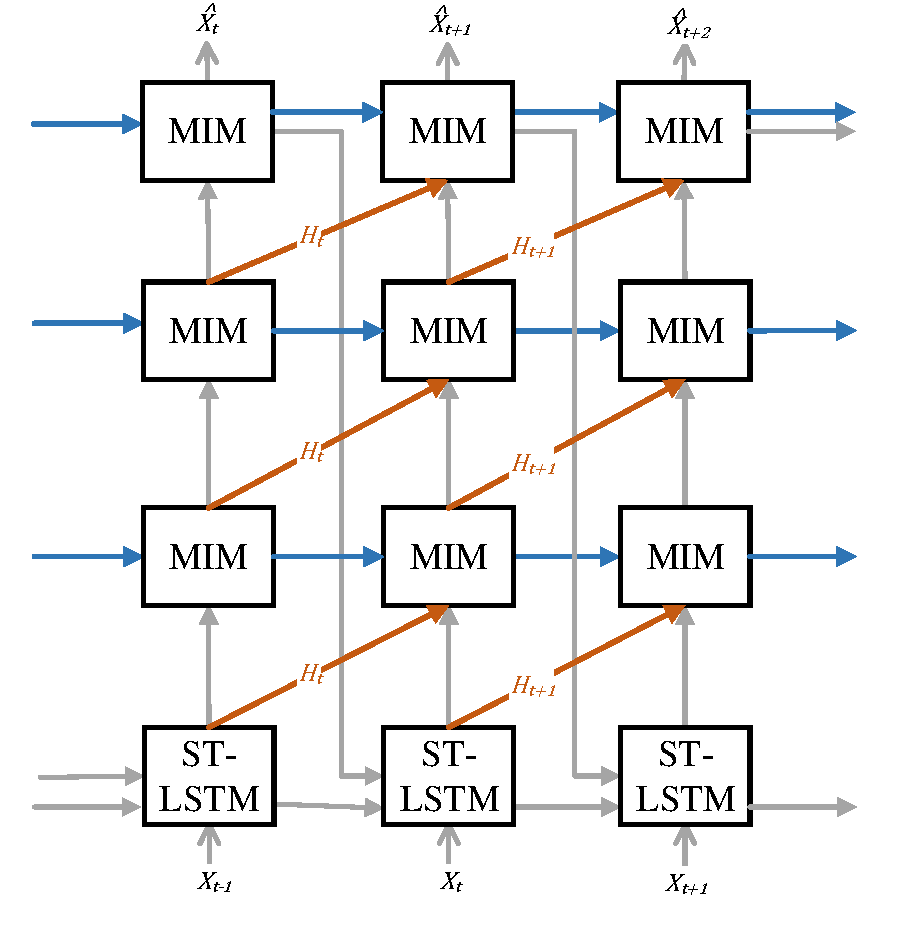
\includegraphics[width=0.5\textwidth]{fig/structure.pdf}
  \caption{The structure of DRNN with $4$ layers. The vertical (gray) arrows denote the zigzag information flows of the spatiotemporal memory $\mathcal{M}$ designed in PredRNN; the diagonal (orange) arrows are added to further deliver the hidden states to generate differential features $\mathcal{D}$; and the horizontal (blue) arrows are modified to deliver the temporal memory $\mathcal{C}$ designed in LSTM, as well as the stationary memory $\mathcal{S}$ and non-stationary memory $\mathcal{N}$ designed in the MIM. % and the differential features $\mathcal{D}$ 
  }
  \label{fig:structure}
\end{figure}

As the hidden states in PredRNN can be used as abstract representations of the input video frames, differencing the hidden states of two adjacent time stamps can reveal the variations of two input frames more evidently. Compared with PredRNN, a node at time stamp $t \neq 1$ and layer $l \neq 1$ takes the hidden state $\mathcal{H}_{t-1}^{l-1}$ from the node at time stamp $t-1$ and layer $l-1$ as extra inputs. These connections are shown as orange arrows in Figure \ref{fig:structure}. As the first layer doesn't have any previous layer, we simply use ST-LSTM \citep{wang2017predrnn} to generate its hidden presentations. Note that, the temporal differencing is performed by subtracting hidden state $\mathcal{H}_{t-1}^{l-1}$ from the hidden state $h_t^{l-1}$ in MIM. As mentioned before, the Memory In Memory (MIM) block has two cascaded temporal memory units to capture the stationary and the non-stationary dynamics respectively. Thus, we modify the horizontal (blue) arrows from PredRNN to further deliver the two temporal memories (denoted by $\mathcal{S}$ for stationary memory and $\mathcal{N}$ for non-stationary memory), as well as the learned differential representations (denoted by $\mathcal{D}$) from the previous time stamp.

\subsection{Memory In Memory}

\begin{figure*}[h]
  \centering
  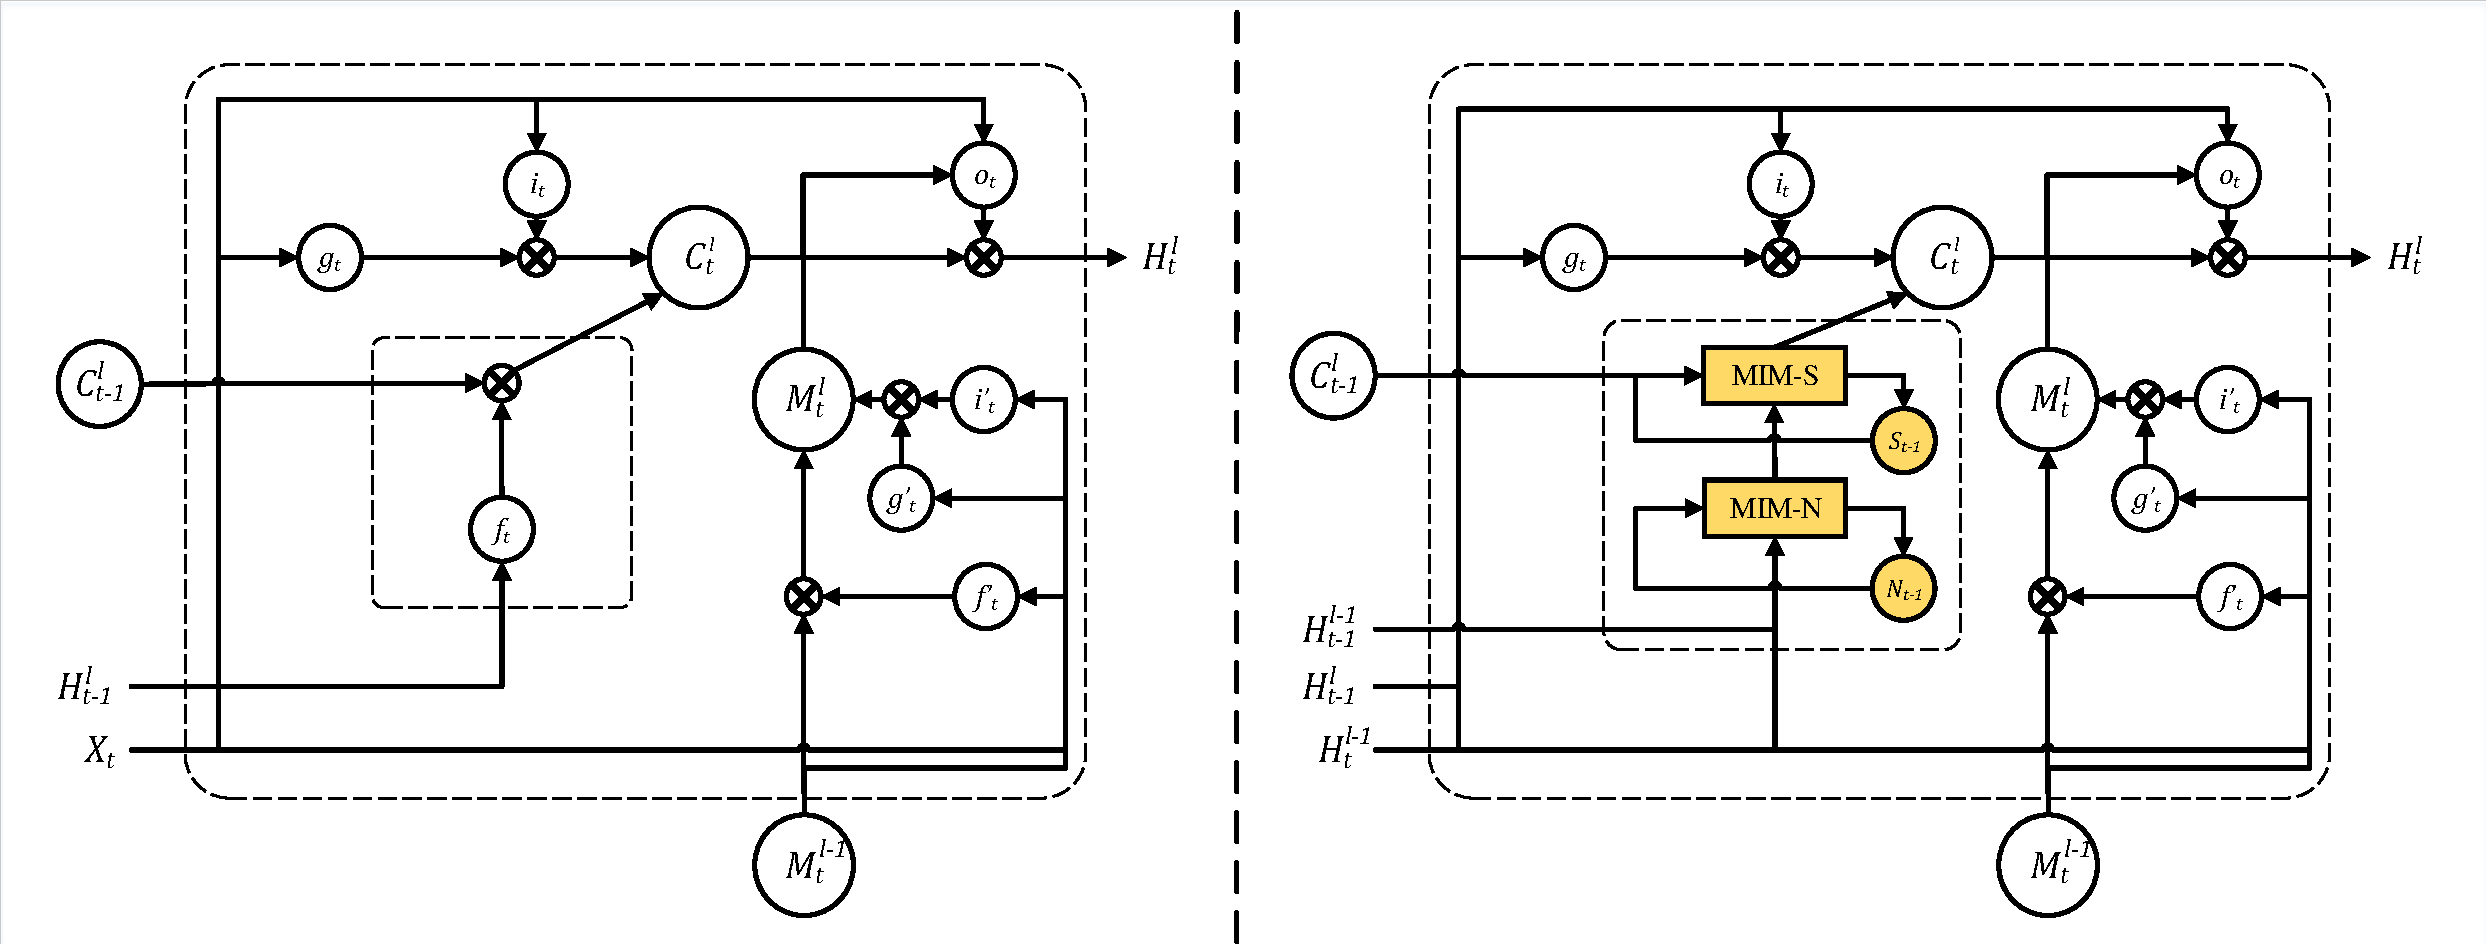
\includegraphics[width=\textwidth]{fig/node.pdf}
  \caption{The ST-LSTM block \citep{wang2017predrnn} in the left plot and the proposed Memory In Memory (MIM) block in the right plot. MIM is designed to introduce two recurrent units (yellow squares) to replace the forget gate (dashed box) in ST-LSTM. MIM-S denotes the stationary unit and MIM-N denotes the non-stationary unit. Note that the MIM block cannot be used in the first layer so the input $\mathcal{X}_t$ is replaced by $\mathcal{H}_t^{l-1}$.}
  \label{fig:node}
\end{figure*}

Our observation is that, the complex dynamics in spatiotemporal sequences can be handled more effectively as a combination of stationary variations and non-stationary variations. Suppose we have a spatiotemporal sequence showing a walking man for example. The speed of the man can be seen as stationary variation and the swing of the man's arms should be considered as non-stationary variation, which we should make more effort to model them. Unfortunately, the forget gate in vanilla LSTM and ST-LSTM is a simple gating structure that struggles to capture the non-stationary variations in spatiotemporal sequences. In our preliminary experiments, we find that the majority of forget gates in the PredRNN model \citep{wang2017predrnn} are saturated, implying that the units always remember similar variations. In another word, what is learned is mainly the stationary component. 

The Memory In Memory (MIM) block is enlightened by the idea of modeling the non-stationary variations using a series of cascaded memory transitions instead of the simple, saturation-prone forget gate in ST-LSTM. As compared in Figure \ref{fig:node} (the dashed boxes), two cascaded temporal memory recurrent units are designed to replace the temporal forget gate $f_t$ in ST-LSTM. The first unit additionally taking $\mathcal{H}_{t-1}^{l-1}$ as input is used to capture the non-stationary variations based on the differencing $(\mathcal{H}_{t-1}^{l-1} - \mathcal{H}_t^{l-1})$ between two consecutive frames, so we name it \textbf{non-stationary unit} (shown as \textbf{MIM-N} in Figure \ref{fig:node}). The non-stationary unit generates differential features $\mathcal{D}_t^l$ based on the difference-stationary assumption \citep{percival1993spectral}. 
%The second unit taking the differential features $\mathcal{D}_t^l$ as input captures the general variations in spatiotemporal sequences, that is, the stationary variations. 
The other unit takes as inputs the output $\mathcal{D}_t^l$ of the non-stationary unit and the temporal memory $\mathcal{C}_{t}^{l-1}$ of the outer ST-LSTM to capture the general stationary variations in spatiotemporal sequences, so we call it \textbf{stationary unit} (shown as \textbf{MIM-S} in Figure \ref{fig:node}). 

\begin{figure}[h]
  \centering
  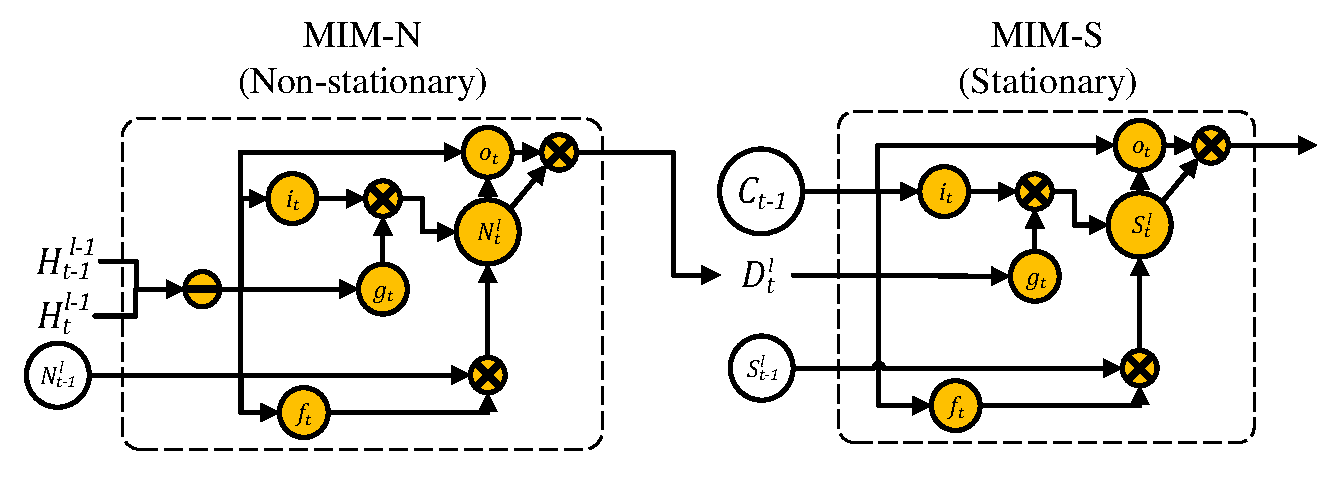
\includegraphics[width=0.5\textwidth]{fig/units.pdf}
  \caption{Non-stationary unit (MIM-N) and stationary unit (MIM-S), which are organized in a cascade structure in the MIM block. Note that non-stationary variation is modeled by sequence differencing.}
  \label{fig:subunits}
\end{figure}

It is important to emphasize that, by differencing the consecutive frames, the non-stationary variations are made more prominent while the stationary variations are significantly suppressed. Thus, the non-stationary unit will not memorize much information from the previous state. By replacing the forget gate in ST-LSTM with the output of the cascaded non-stationary and stationary units (as shown in Figure~\ref{fig:node}), the non-stationary dynamics can be captured more effectively. Key calculations inside a MIM unit can be shown as follows:
\begin{equation}\label{equ:MIM}
  \small
  \begin{split}
  & g_t = \tanh(W_{xg} \ast \mathcal{H}_t^{l-1} + W_{hg} \ast \mathcal{H}_{t-1}^l + b_g) \\
  & i_t = \sigma(W_{xi} \ast \mathcal{H}_t^{l-1} + W_{hi} \ast \mathcal{H}_{t-1}^l + b_i) \\
  & \mathcal{D}_t^l = \text{MIM-N}(\mathcal{H}_t^{l-1}, \mathcal{H}_{t-1}^{l-1}, \mathcal{N}_{t-1}^l) \\
  & \mathcal{C}_t^l = \text{MIM-S}(\mathcal{D}_t^l, \mathcal{C}_{t-1}^l, \mathcal{S}_{t-1}^l) + i_t \odot g_t \\
  & g_t^\prime = \tanh(W_{xg}^\prime \ast \mathcal{H}_t^{l-1} + W_{mg} \ast \mathcal{M}_t^{l-1} + b_g^\prime) \\
  & i_t^\prime = \sigma(W_{xi}^\prime \ast \mathcal{H}_t^{l-1} + W_{mi} \ast \mathcal{M}_t^{l-1} + b_i^\prime) \\
  & f_t^\prime = \sigma(W_{xf}^\prime \ast \mathcal{H}_t^{l-1} + W_{mf} \ast \mathcal{M}_t^{l-1} + b_f^\prime) \\
  & \mathcal{M}_t^l = f_t^\prime \odot \mathcal{M}_t^{l-1} + i_t^\prime \odot g_t^\prime \\
  & o_t = \sigma(W_{xo} \ast \mathcal{H}_t^{l-1} + W_{ho} \ast \mathcal{H}_{t-1}^l + W_{co} \ast \mathcal{C}_t^l + W_{mo} \ast \mathcal{M}_t^l + b_o) \\ 
  & \mathcal{H}_t^l = o_t \odot \tanh(W_{1\times1} \ast [\mathcal{C}_t^l, \mathcal{M}_t^l]),\\
  \end{split}
\end{equation}
where MIM-N and MIM-S denote the stationary unit and the non-stationary unit respectively; $\mathcal{S}$ and $\mathcal{N}$ denote the horizontally-transited memory cells in the two corresponding recurrent units; $\mathcal{D}$ denotes the differential features, which are learned by the non-stationary unit and fed into the stationary unit. The cascade structure enables end-to-end modeling of both stationary and non-stationary dynamics.

%As we know, the hidden representations tend to learn more general rules of variations, that is, the stationary variations. That's why the results of predictive learn tend to become blurred. The stationary unit takes differences of hidden representations as input and outputs $\mathcal{D}$ which contains stationary variational features. So that the non-stationary unit can pay more attention to non-stationary variations. 

A schematic of the stationary and non-stationary units is presented in Figure \ref{fig:subunits}. We present the detailed calculations of the non-stationary unit (MIM-N) as follows:
\begin{equation}\label{equ:stationary}
  \small
  \begin{split}
  & g_t = \tanh(W_{xg} \ast (\mathcal{H}_t^{l-1} - \mathcal{H}_{t-1}^{l-1}) + W_{ng} \ast \mathcal{N}_{t-1}^l + b_g) \\
  & i_t = \sigma(W_{xi} \ast (\mathcal{H}_t^{l-1} - \mathcal{H}_{t-1}^{l-1}) + W_{ni} \ast \mathcal{N}_{t-1}^l + b_i)\\
  & f_t = \sigma(W_{xf} \ast (\mathcal{H}_t^{l-1} - \mathcal{H}_{t-1}^{l-1}) + W_{nf} \ast \mathcal{N}_{t-1}^l + b_f) \\
  & \mathcal{N}_t^l = f_t \odot \mathcal{N}_{t-1}^l + i_t \odot g_t \\
  & o_t = \sigma(W_{xo} \ast (\mathcal{H}_t^{l-1} - \mathcal{H}_{t-1}^{l-1}) + W_{no} \ast \mathcal{N}_t^l + b_o) \\ 
  & \text{MIM-N}(\mathcal{H}_t^{l-1}, \mathcal{H}_{t-1}^{l-1}, \mathcal{N}_{t-1}^l) = o_t \odot \tanh(\mathcal{N}_t^l),\\
  \end{split}
\end{equation}
where all gates $g_t$, $i_t$, $f_t$ and $o_t$ are updated by the frame difference $(\mathcal{H}_t^{l-1} - \mathcal{H}_{t-1}^{l-1})$, which highlights the non-stationary variations in the spatiotemporal sequence, and focuses the unit more on the non-stationary dynamics.
%where $\mathcal{D}$ is also delivered vertically so that the stationary unit can capture the general trend of spatiotemporal sequences better. The gates $g_t$, $i_t$, $f_t$ and $o_t$ gives the stationary unit ability to memory. It can update the stationary memory $\mathcal{S}$ based on the differential information $(\mathcal{H}_{t-1}^{l-1} - \mathcal{H}_t^{l-1})$. And then generate a new stationary variations feature $\mathcal{D}_t^l$. And the calculations of the non-stationary units are shown as below:

Similarly, the detailed calculations of the stationary unit (MIM-S) are shown as follows:
\begin{equation}\label{equ:non-stationary}
  \small
  \begin{split}
  & g_t = \tanh(W_{dg} \ast \mathcal{D}_t^l + W_{cg} \ast \mathcal{C}_{t-1}^l + b_g) \\
  & i_t = \sigma(W_{di} \ast \mathcal{D}_t^l + W_{ci} \ast \mathcal{C}_{t-1}^l + b_i)\\
  & f_t = \sigma(W_{df} \ast \mathcal{D}_t^l + W_{cf} \ast \mathcal{C}_{t-1}^l + b_f) \\
  & \mathcal{S}_t^l = f_t \odot \mathcal{S}_{t-1}^l + i_t \odot g_t \\
  & o_t = \sigma(W_{do} \ast \mathcal{D}_t^l + W_{co} \ast \mathcal{C}_{t-1}^l + W_{so} \ast \mathcal{S}_t^l + b_o) \\ 
  & \text{MIM-S}(\mathcal{D}_t^l, \mathcal{C}_{t-1}^l, \mathcal{S}_{t-1}^l) = o_t \odot \tanh(\mathcal{S}_t^l),\\
  \end{split}
\end{equation}
which takes the memory states $\mathcal{C}_{t-1}^l$ and the differential features $\mathcal{D}_{t-1}^l$ of MIM-N as input. As can be validated, the stationary unit provides a gating mechanism to adaptively decide whether to trust the original memory or the differential feature of MIM-N. If the differential features vanish, indicating that the non-stationary dynamics is not prominent, then the unit will mainly reuse the original memory. Otherwise, if the differential features are prominent, then the unit will overwrite the memory to focus more on the non-stationary dynamics. 

%which is similar with the stationary unit. Note that the hidden states in the non-stationary unit is $\mathcal{C}_{t-1}^l$, which will be updated in the non-stationary unit. The non-stationary unit updates $\mathcal{C}$ based on $\mathcal{D}_t^l$ and $\mathcal{C}_{t-1}^l$. It pays more attention on non-stationary variations while the stationary variations are ready. The output discards information more accurately and will be merged with the result of the input gate of MIM. As for network details, the MIM in the first time stamp do not have any previous hidden representations as input, so the stationary unit takes a matrix filled with zero as initialization.

%------------------------------------------------------------------------
\section{Experiments}
\label{sec:Experiments}
In this section, we perform extensive evaluation of the proposed Memory in Memory (MIM) approach. For each evaluation dataset, we will introduce the dataset details and the implementation details of our proposed approach on it. At last, we report the performance of our MIM model and analyze experimental results both qualitatively and quantitatively.

We use three video prediction datasets: a synthetic dataset with moving digits, a real video dataset with human actions and a standard traffic flow prediction dataset. Our model has $4$ layers in all experiments, including a ST-LSTM layer as the first layer and three MIM blocks. The number of channels in each MIM block is $64$, as a balance of prediction accuracy and memory cost efficiency. We train all of the models with L2 loss, using the ADAM optimizer \citep{Kingma2014Adam} with a $0.001$ starting learning rate. The training process is stopped after $100,000$ iterations. The batch size of each iteration is set to $8$. Note that we extend the layer normalization \citep{Ba2016Layer} to 3D tensors and apply it on the MIM and ConvLSTM models, based on the idea that the training process of deep convolutional networks can be stabilized by reducing the covariate shift problem \citep{ioffe2015batch}. Note that the MIM blocks in the first time stamp do not have any previous hidden representations as input, so the non-stationary units take matrices filled with zero as initialization. All experiments are implemented in TensorFlow \citep{Abadi2016TensorFlow}.

\textbf{Baseline Models:} We mainly focus the comparative study with the following state-of-the-art methods: \textbf{ConvLSTM} \citep{shi2015convolutional} is the first deep network that uses convolution in LSTM and shows great results on video prediction;
\textbf{FRNN} Oliu \textit{et al.} \citep{oliu2017folded} uses ConvGRU units and shares states to avoid re-encoding of the predictions. The ConvGRU nodes from encoder do not share weights with the nodes from decoder in this method, which is inherited from the encoder-predictor recurrent architecture \citep{Sutskever2014Sequence,Cho2014On};
\textbf{VPN} \citep{Kalchbrenner2016Video} has shown a great performance in many video prediction tasks. As a strong competitor, we include VPN model to demonstrate the importance of exploiting the differential patterns and the cascaded memory recurrent units.

\subsection{Moving MNIST Dataset}

\paragraph{Implementation} Moving MNIST dataset consists of $64 \times 64 \times 1$ grayscale sequences of length $20$ displaying pairs of digits moving around the image (10 for the inputs and 10 for the predictions). The sequences are generated by the method described in the work of Srivastava \textit{et al.} \citep{srivastava2015unsupervised}, following the experimental settings in PredRNN \citep{wang2017predrnn}. Before training the model, we apply max-min normalization to scale the data from its original intensities to $[0, 1]$. In particular, to reduce the training time and memory usage on the Moving MNIST dataset, we reshape each $64 \times 64 \times 1$ input image into a $16 \times 16 \times 16$ tensor. By doing this, we significantly reduce the parameters and training time of MIM, while the performance is affected marginally. Besides, the scheduled sampling strategy \citep{bengio2015scheduled} is applied to all of the models to stitch the discrepancy between training and inference.

\begin{table}[h]
  \caption{A comparison for predicting $10$ frames on the moving MNIST dataset. All of the models are trained with $10$ target frames and have comparable numbers of parameters.}
  \label{tab:mnist_10_result}
  \vskip 0.15in
  \centering
  \begin{small}
  \begin{sc}
  \renewcommand{\multirowsetup}{\centering}  
  \begin{tabular}{lccc}
    \toprule
    Model & SSIM & MSE & MAE\\
    \midrule
    FC-LSTM & 0.690 & 118.3 & 209.4 \\ 
    CONVLSTM & 0.707 & 103.3 & 182.9 \\ 
    TrajGRU & 0.713 & 106.9 & 190.1 \\ 
    CDNA & 0.721 & 97.4 & 175.3 \\ 
    DFN & 0.726 & 89.0 & 172.8 \\ 
    FRNN & 0.813 & 69.7 & 150.3 \\ 
    VPN & 0.870 & 64.1 & 131.0 \\
    PredRNN & 0.867 & 56.8 & 126.1 \\
    \midrule
    \textbf{MIM} & \textbf{0.874} & \textbf{52.0} & \textbf{116.5} \\
    \bottomrule
  \end{tabular}
  \end{sc}
  \end{small}
\end{table}

\begin{table}[h]
  \caption{Ablation study of the MIM block with either stationary unit or non-stationary unit removed. These experiments also predict $10$ frames on the moving MNIST dataset.}
  \label{tab:mnist_10_result_self}
  \vskip 0.15in
  \centering
  \begin{small}
  \begin{sc}
  \renewcommand{\multirowsetup}{\centering}  
  \begin{tabular}{lccc}
    \toprule
    Model & SSIM & MSE & MAE\\
    \midrule
%    Multi-task learning \\
%    Input difference to ST-LSTM\\
    MIM (without MIM-N) & 0.858 & 54.4 & 124.8 \\
    MIM (without MIM-S) & 0.853 & 55.7 & 125.5 \\
    \midrule
    \textbf{MIM} & \textbf{0.874} & \textbf{52.0} & \textbf{116.5} \\
    \bottomrule
  \end{tabular}
  \end{sc}
  \end{small}
\end{table}

\paragraph{Results} We measure the per-frame structural similarity index measure (SSIM) \citep{Wang2004Image}, the mean square error (MSE) and the mean absolute error (MAE) to evaluate our models, as shown in table \ref{tab:mnist_10_result}. A lower RMSE or MAE denotes better prediction performance, so does a higher SSIM. Additionally, we also include FC-LSTM \citep{srivastava2015unsupervised}, TrajGRU \citep{shi2017deep}, CDNA \citep{Finn2016Unsupervised} and DFN \citep{de2016dynamic} for comparison. MIM reduces the former best MSE and MAE results to $52.1$ and $120.8$ respectively. The SSIM result also reaches $0.874$. We also design two ablation experiments, by respectively removing the stationary units or non-stationary units, to verify necessity of the cascaded temporal memory recurrent units. As table \ref{tab:mnist_10_result_self} shown, non-stationary units work better than stationary units and they work best when they are cascaded.

The sequences in Moving MNIST dataset have less variations as they are generated by two moving digits with fixed speed. To verify that our model can capture the variations (especially non-stationary variations) better, we add different acceleration to the speed and generate a new Moving MNIST dataset with variant speed. The results of PredRNN \citep{wang2017predrnn}, PredRNN++ \citep{wang2018predrnn++} and MIM are shown as table \ref{tab:mnist_a_10_result_self}. These experiments also predict 10 frames based on 10 observations. Obviously, MIM achieves better performence on datasets which have more variations.

\begin{table}[h]
  \caption{A comparison for predicting $10$ frames on the moving MNIST dataset with acceleration. All of the models are also trained with $10$ target frames and have comparable numbers of parameters.}
  \label{tab:mnist_a_10_result_self}
  \vskip 0.15in
  \centering
  \begin{small}
  \begin{sc}
  \renewcommand{\multirowsetup}{\centering}  
  \begin{tabular}{lccc}
    \toprule
    Model & SSIM & MSE & MAE\\
    \midrule
%    Multi-task learning \\
%    Input difference to ST-LSTM\\
    PredRNN & 0. & 0. & 0. \\
    PredRNN++ & 0. & 0. & 0. \\
    \midrule
    \textbf{MIM} & \textbf{0.} & \textbf{0.} & \textbf{0.} \\
    \bottomrule
  \end{tabular}
  \end{sc}
  \end{small}
\end{table}

\begin{figure}[h]
  \centering
  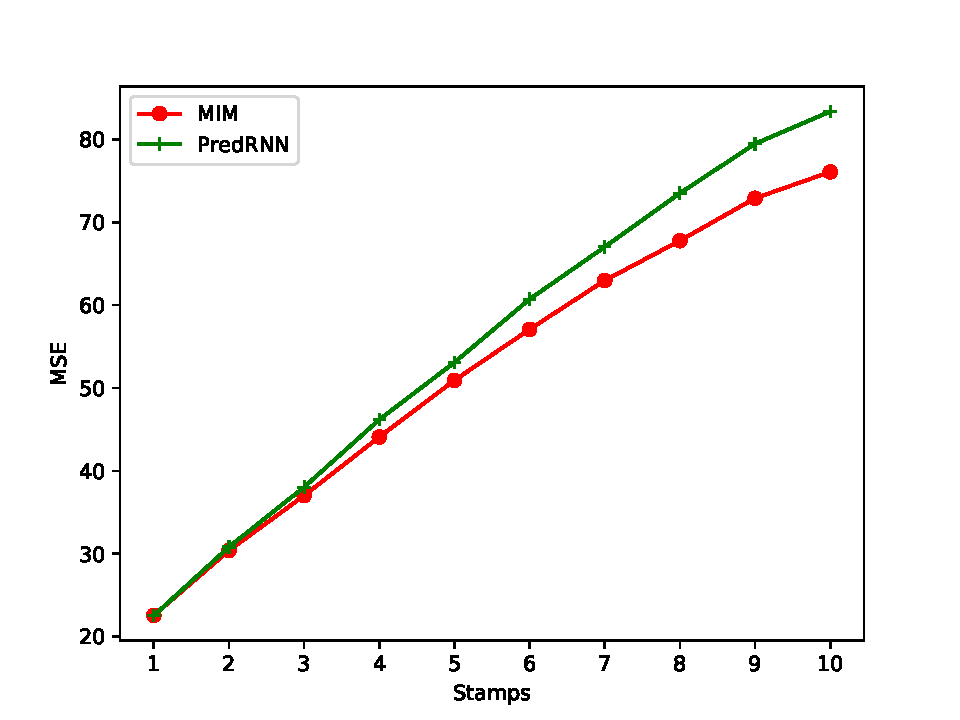
\includegraphics[width=0.4\textwidth]{fig/mnist.pdf}
  \caption{Frame-wise MSE over the MNIST test sets. Lower curves denote higher accuracy.}
  \label{fig:mnist_mse}
\end{figure}

\begin{figure}[h]
  \centering
  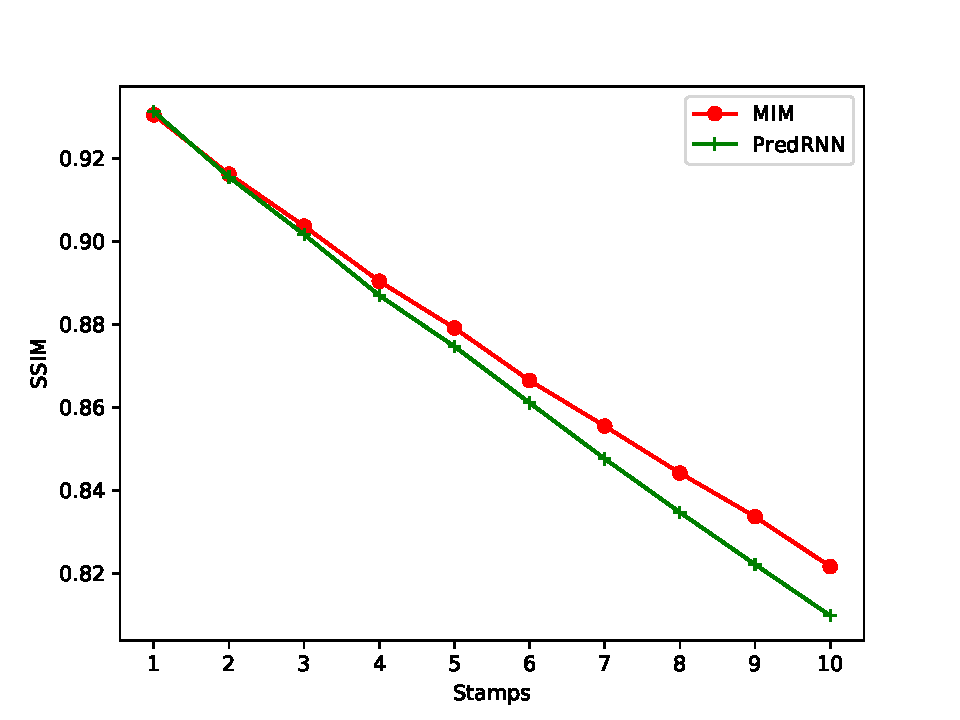
\includegraphics[width=0.4\textwidth]{fig/mnist_ssim.pdf}
  \caption{Frame-wise SSIM over the MNIST test sets. Higher curves denote higher accuracy.}
  \label{fig:mnist_ssim}
\end{figure}

%In Figure \ref{fig:mnist_results}, we visualize the corresponding generated images. The predictions of FRNN are vague, while PredRNN and MIM are better. Note that MIM predicts the shape of the digits better, such as the upper part of the digit "7". Figure \ref{fig:mnist_mse} shows the frame-wise MSE of 2 models (PredRNN and MIM) over the test sets. As the number of predicted frames grows, the curve of MIM gets lower, indicating that our cascaded temporal memory forget structure is necessary. Figure \ref{fig:mnist_ssim} confirms the same conclusion, which shows the frame-wise SSIM of PredRNN and MIM.

\begin{figure}[h]
  \centering
  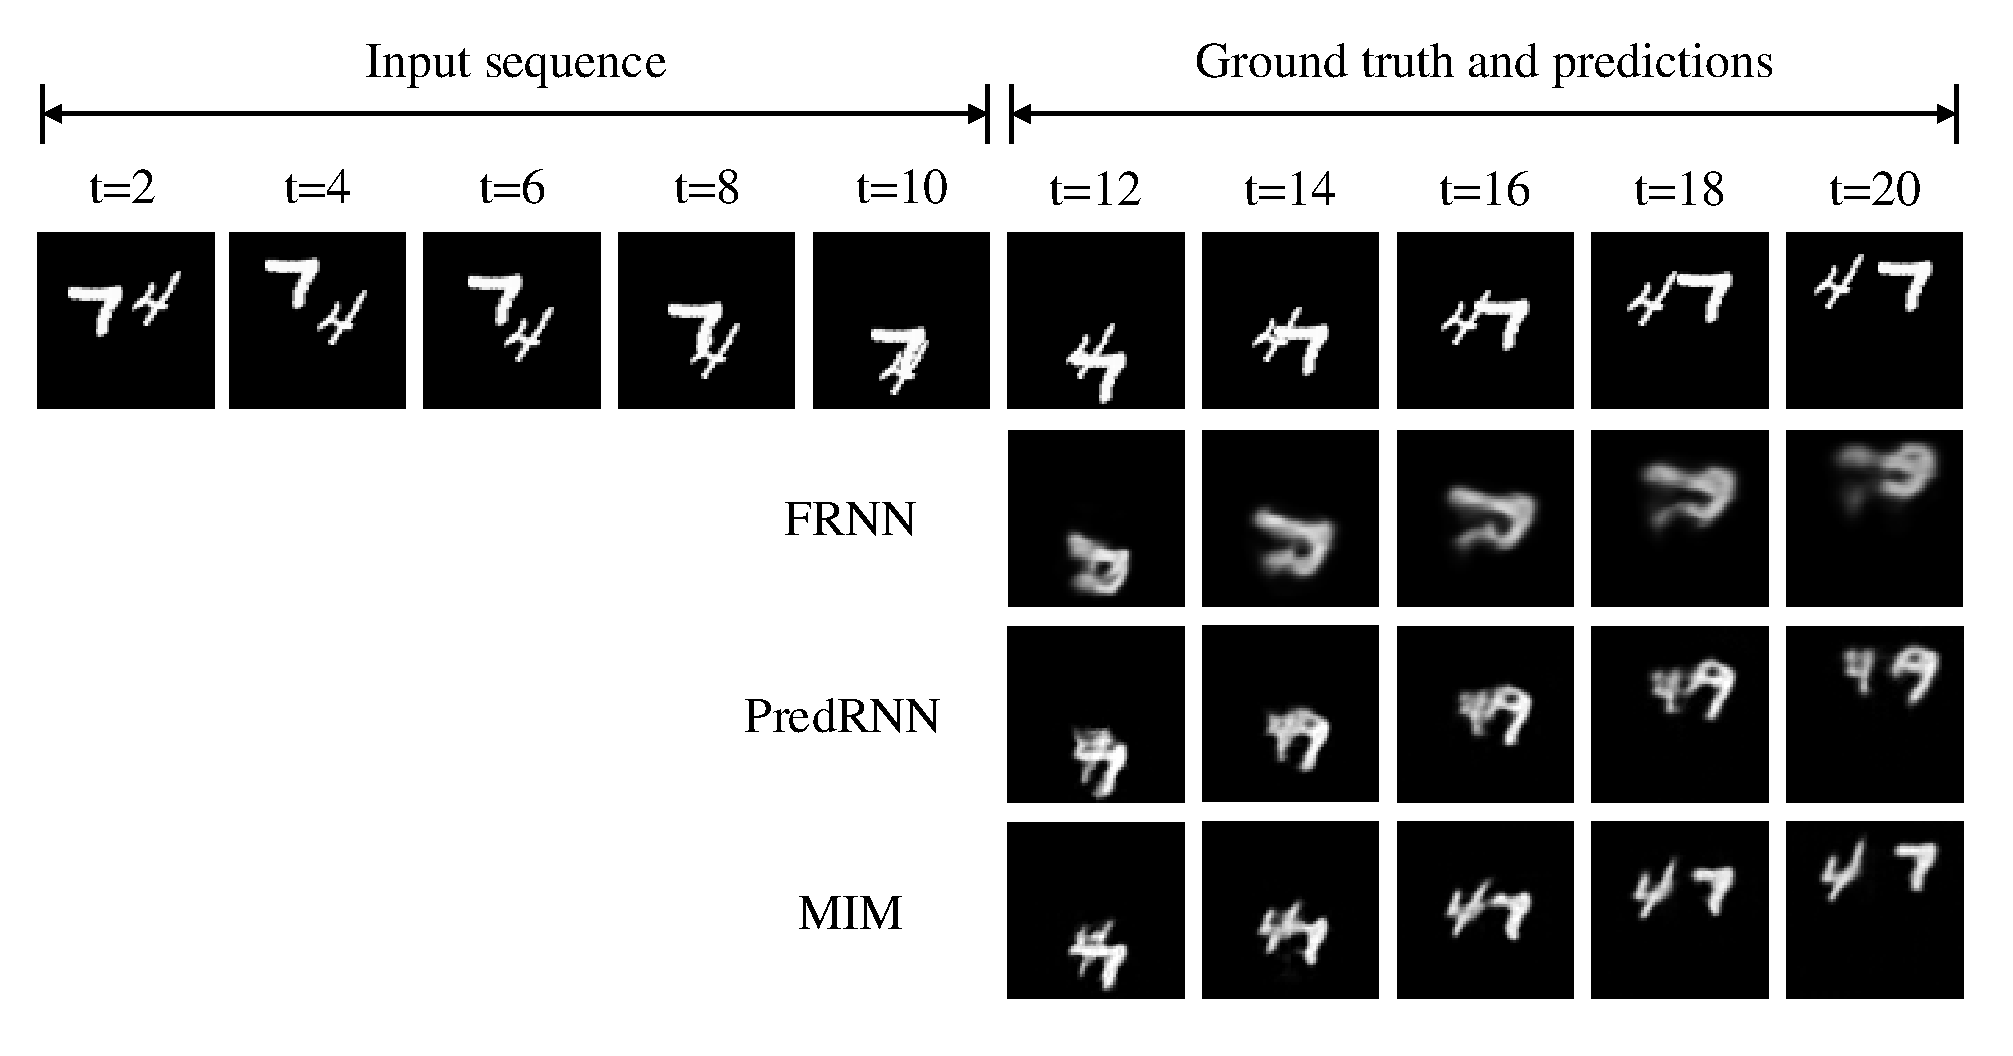
\includegraphics[width=0.5\textwidth]{fig/mnist_predictions.pdf}
  \caption{A demonstration of predictions on moving MNIST test set. All models predict 10 frames into the future by observing 10 frames. Frames are shown at a two frames interval.}
  \label{fig:mnist_results}
\end{figure}

In Figure \ref{fig:mnist_results}, we visualize the corresponding generated images. The predictions of FRNN are blurred, while PredRNN and MIM are better. Note that MIM predicts the shapes of the digits better, such as the upper part of the digit ``7''. Figure \ref{fig:mnist_mse} shows the frame-wise MSE of 2 models (PredRNN and MIM) over the test sets. As the number of predicted frames grows, the curve of MIM gets lower, indicating that our cascaded temporal memory recurrent units are necessary. Figure \ref{fig:mnist_ssim} shows the frame-wise SSIM of PredRNN and MIM, which confirms the same conclusion.


\subsection{KTH Action Dataset}

\paragraph{Implementation} KTH consists of 600 videos of 15-20 seconds with 25 persons performing 6 human actions. Each frame in these sequences is grayscale and with the size of $120 \times 160 \times 1$, which will be resized into shapes of $128 \times 128 \times 1$ pixels. The dataset has been split into persons 1 to 16 for training, and 17 to 25 for testing, also following the experimental settings in \cite{wang2017predrnn}. In particular, all of the models are trained to generate subsequent 10 frames from prior 10 frames, and tested to predict 20 frames from 10 frames. We also apply max-min normalization to scale the data from the its original intensities to $[0, 1]$ and reshape each $128 \times 128 \times 1$ input image into a $32 \times 32 \times 16$ tensor in the same way as we did on moving MNIST dataset. The scheduled sampling strategy \citep{bengio2015scheduled} is also applied to the experiments on KTH action dataset.

\begin{table}[h]
  \caption{A comparison for predicting $20$ frames on the KTH action dataset. All of the models are trained with $10$ target frames and made to predict $20$ future frames at test time. They have comparable numbers of parameters.}
  \label{tab:kth_20_result}
  \vskip 0.15in
  \centering
  \begin{small}
  \begin{sc}
  \renewcommand{\multirowsetup}{\centering}  
  \begin{tabular}{lcc}
    \toprule
    Model & PSNR & SSIM\\
    \midrule
    CONVLSTM & 23.58 & 0.712 \\ 
    TrajGRU & 26.97 & 0.790 \\ 
    DFN & 27.26 & 0.794 \\ 
    MCNET & 25.95 & 0.804 \\ 
    FRNN & 26.12 & 0.771 \\ 
    PredRNN & 27.55 & 0.801 \\
    \midrule
    \textbf{MIM} & \textbf{28.16} & \textbf{0.806} \\
    \bottomrule
  \end{tabular}
  \end{sc}
  \end{small}
\end{table}

\begin{figure}[h]
  \centering
  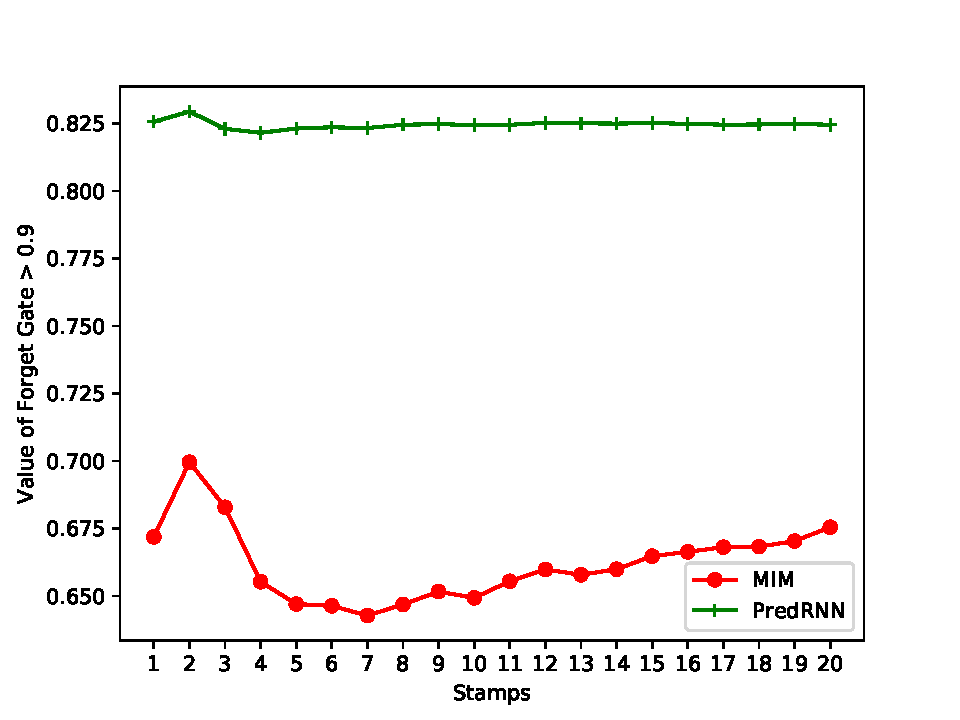
\includegraphics[width=0.4\textwidth]{fig/action.pdf}
  \caption{Percentage of value which greater than 0.9 from the forget gate (KTH dataset).}
  \label{fig:action_forget}
\end{figure}

\paragraph{Results} In the experiments on KTH action dataset, we use image-level PSNR and SSIM to evaluate our models, as shown in table \ref{tab:kth_20_result}. A higher PSNR denotes better prediction performance. We include MCNET \citep{Villegas2017Decomposing} for comparison in these experiments. Note that all of the models are trained with $10$ target frames and predicted $20$ future frames. MIM consistently outperforms the baseline models. Figure \ref{fig:action_results} shows a person running from the near to the distant. Note that the person in the predictions of PredRNN keeps running nearby, while MIM makes the person run far away. To verify the necessity of our cascaded temporal memory recurrent units, we output the value of the forget gate from PredRNN and MIM and calculate the percentage of the value which is greater than 0.9, as shown in Figure \ref{fig:action_forget}. Note that we divide the outputs of the cascaded temporal memory recurrent units by the original cell state to get the ``fake'' forget gate value. Obviously, most of the forget gate value of PredRNN is greater than 0.9, while it is about $60\%$ in MIM. Meanwhile, the value of ``forget gate'' in MIM is more volatile.

As shown in table \ref{tab:kth_20_result}, PredRNN++ \citep{wang2018predrnn++} is still better than MIM. Considering most of the human actions in the KTH Action Dataset are simple, such as walking or jogging. We split the KTH Action Dataset into two subsets based on their variations. (methods). The results of PredRNN \citep{wang2017predrnn}, PredRNN++ \citep{wang2018predrnn++} and MIM on "stationary" KTH dataset are shown in table \ref{tab:KTH_s_20_result}, while the results on "non-stationary" KTH dataset are shown in table \ref{tab:KTH_n_20_result}. These experiments are also trained to generate subsequent 10 frames from prior 10 frames, and tested to predict 20 frames from 10 frames. Obviously, MIM achieves better performence on datasets which have more variations.

\begin{table}[h]
  \caption{A comparison for predicting $20$ frames on the "stationary" KTH action dataset. All of the models are also trained with $10$ target frames and made to predict $20$ future frames at test time.}
  \label{tab:KTH_s_20_result}
  \vskip 0.15in
  \centering
  \begin{small}
  \begin{sc}
  \renewcommand{\multirowsetup}{\centering}  
  \begin{tabular}{lccc}
    \toprule
    Model & SSIM & MSE & MAE\\
    \midrule
%    Multi-task learning \\
%    Input difference to ST-LSTM\\
    PredRNN & 0. & 0. & 0. \\
    PredRNN++ & 0. & 0. & 0. \\
    \midrule
    \textbf{MIM} & \textbf{0.} & \textbf{0.} & \textbf{0.} \\
    \bottomrule
  \end{tabular}
  \end{sc}
  \end{small}
\end{table}

\begin{table}[h]
  \caption{A comparison for predicting $20$ frames on the "non-stationary" KTH action dataset. All of the models are also trained with $10$ target frames and made to predict $20$ future frames at test time.}
  \label{tab:KTH_n_20_result}
  \vskip 0.15in
  \centering
  \begin{small}
  \begin{sc}
  \renewcommand{\multirowsetup}{\centering}  
  \begin{tabular}{lccc}
    \toprule
    Model & SSIM & MSE & MAE\\
    \midrule
%    Multi-task learning \\
%    Input difference to ST-LSTM\\
    PredRNN & 0. & 0. & 0. \\
    PredRNN++ & 0. & 0. & 0. \\
    \midrule
    \textbf{MIM} & \textbf{0.} & \textbf{0.} & \textbf{0.} \\
    \bottomrule
  \end{tabular}
  \end{sc}
  \end{small}
\end{table}

\begin{figure}[h]{}
  \centering
  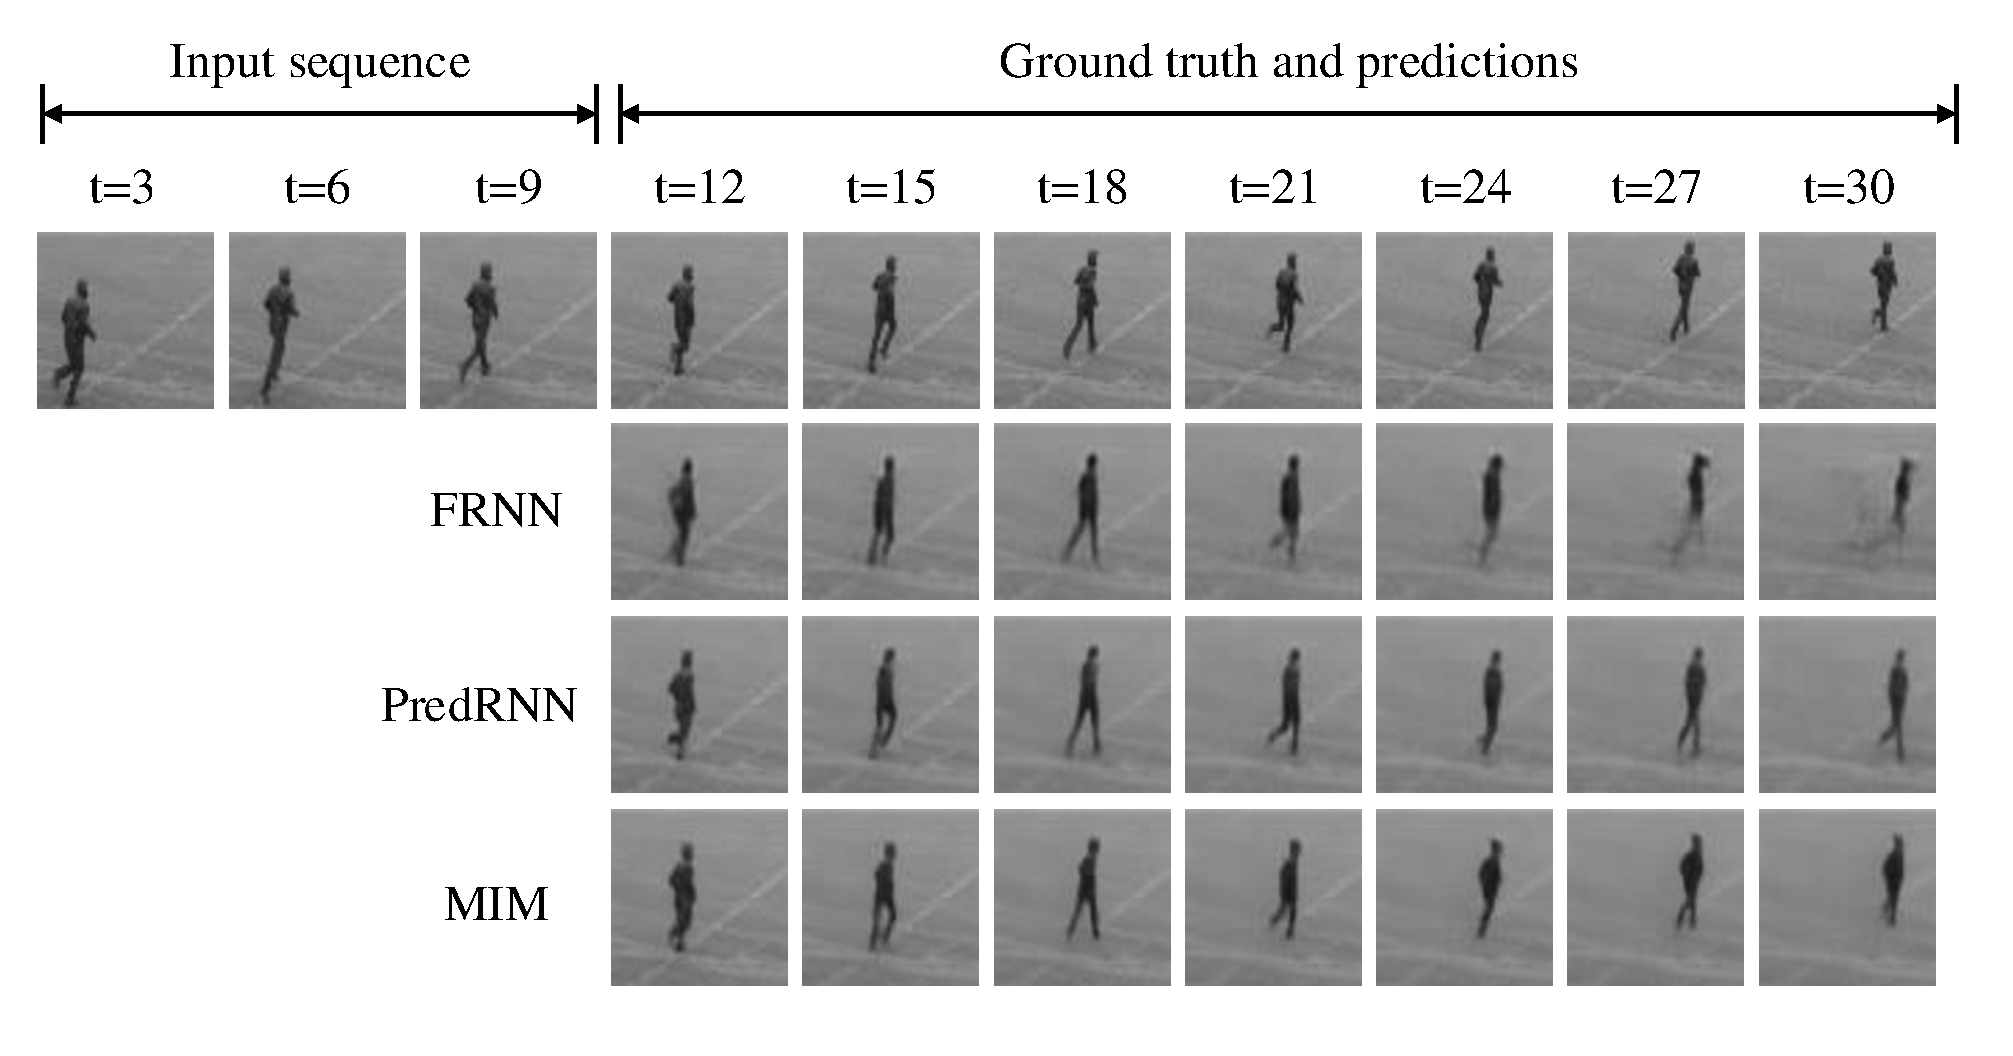
\includegraphics[width=0.5\textwidth]{fig/action_predictions.pdf}
  \caption{A demonstration of predictions on KTH action test set. All models predict 20 frames into the future by observing 10 frames. Frames are shown at a three frames interval.}
  \label{fig:action_results}
\end{figure}


\subsection{TaxiBJ Dataset}

\paragraph{Implementation} TaxiBJ contains traffic flow images collected consecutively from the GPS monitors of taxicabs in Beijing. Each frame in TaxiBJ is a $32 \times 32 \times 2$ grid of image. Two channels represent the traffic flow entering and leaving the same district at this time. We generate sequences from TaxiBJ dataset and split the whole dataset into a training set and a test set as described in the work of Zhang \textit{et al.} \citep{zhang2016dnn}. Each sequence contains 8 consecutive frames, 4 for the inputs and 4 for the predictions. The frames are also scaled to $[0, 1]$ and reshape to $16 \times 16 \times 8$ as described above. Particularly, the scheduled sampling strategy \citep{bengio2015scheduled} is not used in these experiments.

\paragraph{Results} The setting of the experiments on TaxiBJ dataset follows ST-ResNet \citep{zhang2017deep}, which has shown state-of-art results on TaxiBJ dataset. Note that ST-ResNet only predicts one frame in one pass due to its non-recurrent structures. By regarding previous generated images as inputs, we can easily make it predict longer into the future. Compared with PredRNN, MSE of MIM does not decrease much in the first few frames. But as the number of predicted frames increases, the gap becomes larger, shown as table \ref{tab:taxibj_4_result}. Figure \ref{fig:taxibj_results} shows the corresponding generated images on TaxiBJ. For easy observation, we visualize the difference between the predictions and the ground truth images. Obviously, MIM shows good performance in all predicted frames, especially the last few frames.

\begin{table}[h]
  \caption{A comparison of MSE for predicting $4$ frames on the TaxiBJ dataset. All of the models are trained with $4$ target frames and have comparable numbers of parameters}
  \label{tab:taxibj_4_result}
  \vskip 0.15in
  \centering
  \begin{small}
  \begin{sc}
  \renewcommand{\multirowsetup}{\centering}  
  \begin{tabular}{lcccc}
    \toprule
    Model & Frame 1 & Frame 2 & Frame 3 & Frame 4\\
    \midrule
    ST-ResNet & 0.688 & 0.939 & 1.130 & 1.288 \\ 
    VPN & 0.744 & 1.031 & 1.251 & 1.444 \\ 
    FRNN & 0.682 & 0.823 & 0.989 & 1.183 \\ 
    PredRNN & 0.634 & 0.934 & 1.047 & 1.263 \\
    \midrule
    \textbf{MIM} & \textbf{0.554} & \textbf{0.737} & \textbf{0.887} & \textbf{0.999} \\
    \bottomrule
  \end{tabular}
  \end{sc}
  \end{small}
\end{table}

\begin{figure}[h]
  \centering
  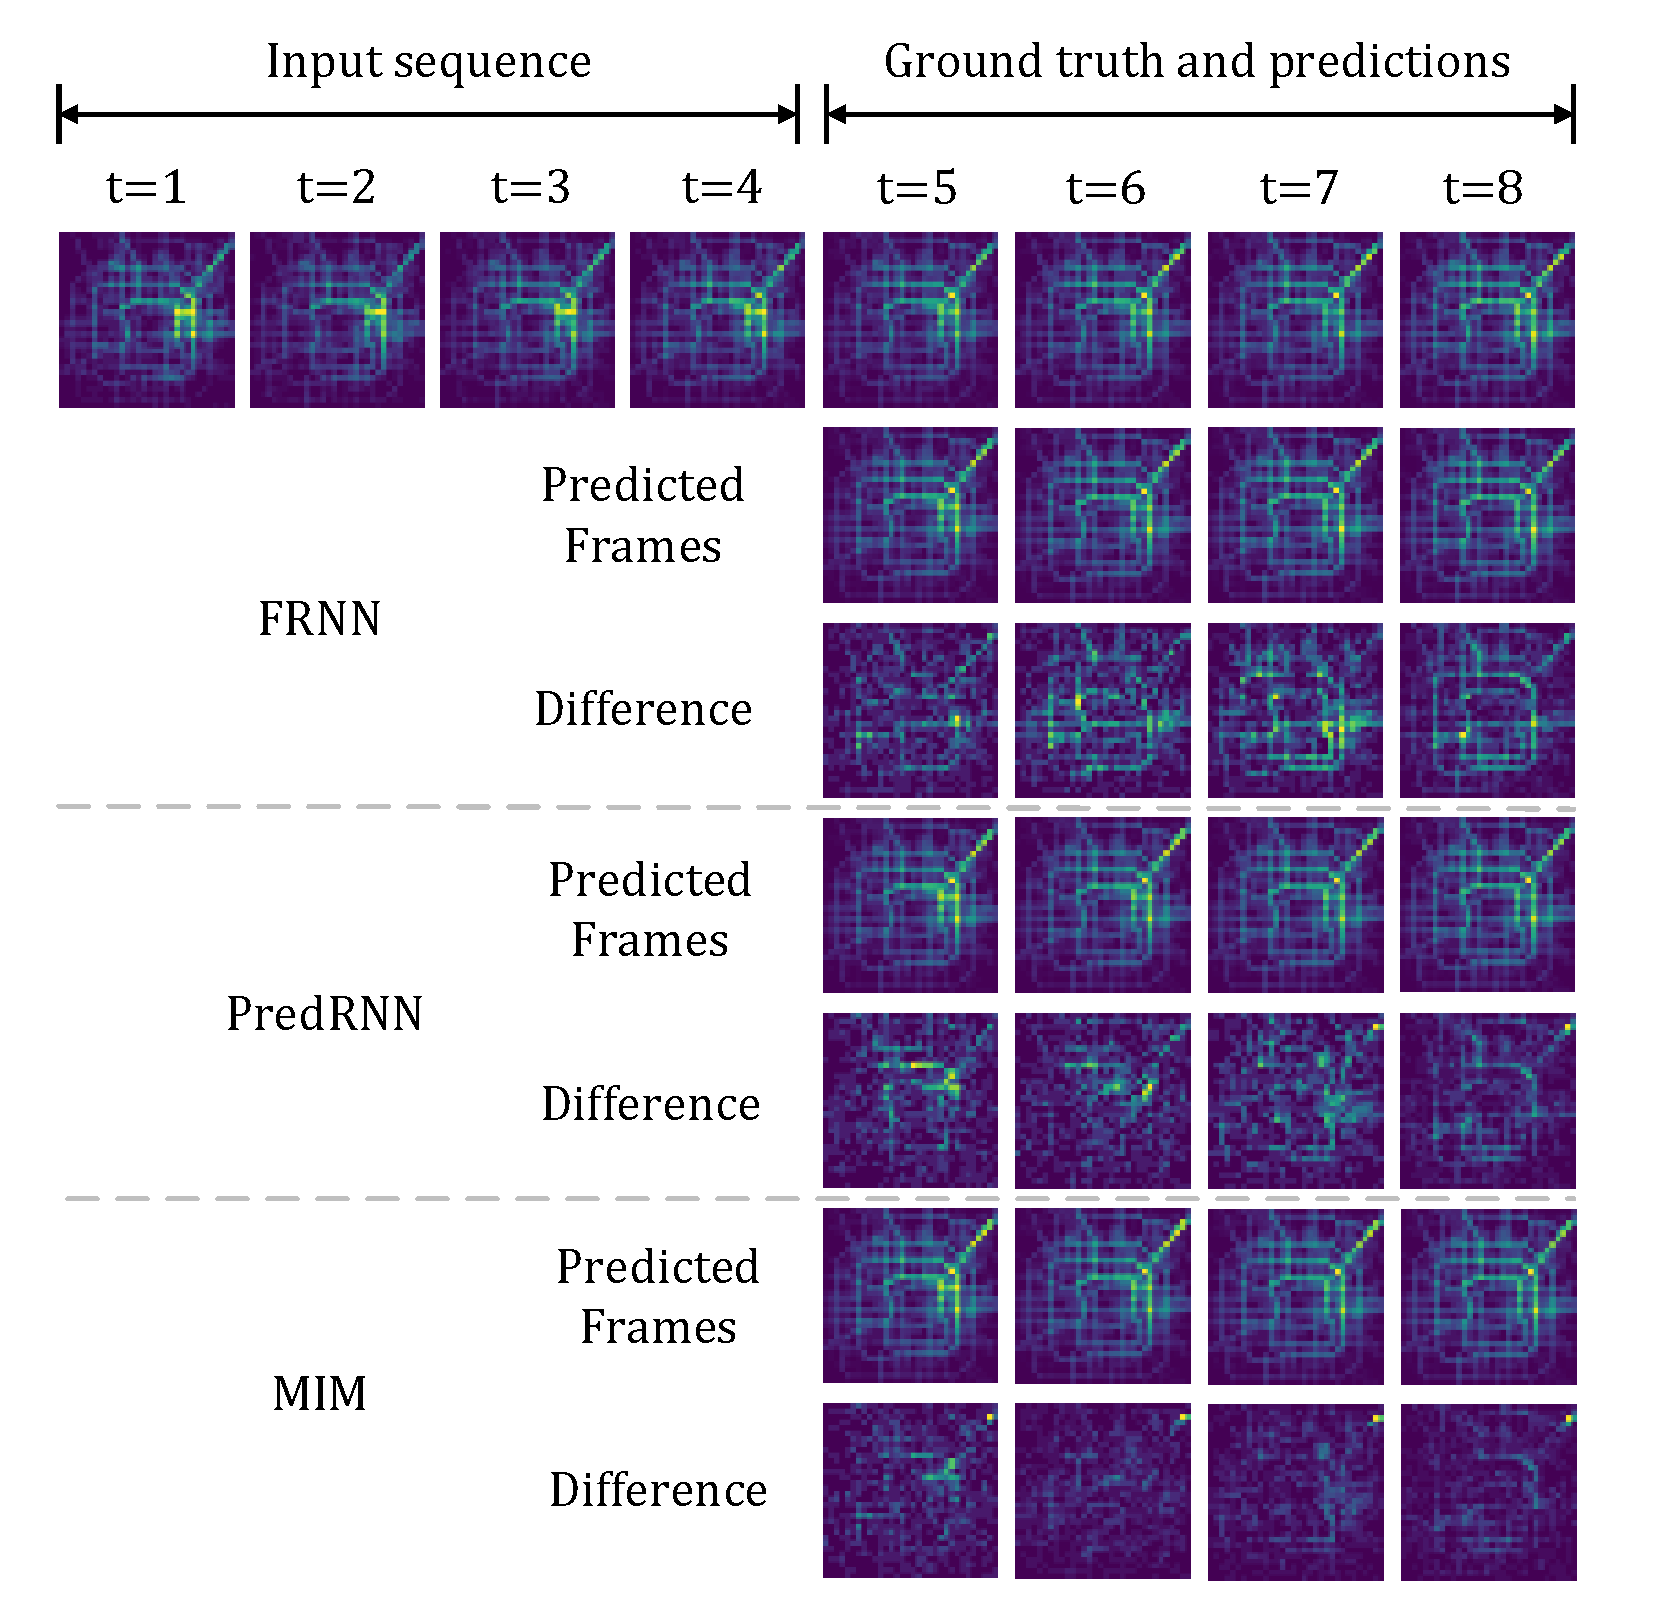
\includegraphics[width=0.5\textwidth]{fig/taxibj.pdf}
  \caption{A demonstration of predictions on TaxiBJ test set. We also visualize the difference between the predictions and the ground truth images for easy observation}
  \label{fig:taxibj_results}
\end{figure}

\section{Conclusions}

We investigates the non-stationarity underlying the spatiotemporal sequences, which forms the main obstacle in spatiotemporal predictive learning. Modern recurrent networks are powerful for modeling stationary sequences, while the attention mechanism has been introduced to model the non-stationary patterns. However, in spatiotemporal predictive learning, the attention mechanism proves less effective. This paper enables non-stationary modeling in video prediction by a differential recurrent neural network taking advantages of the differential information between adjacent recurrent states. A Memory In Memory (MIM) block is derived to model the spatiotemporal variations, which uses two cascaded memory recurrent units to handle non-stationary and stationary spatiotemporal variations respectively. MIM achieves the state-of-the-art prediction performance on three video datasets: a synthetic dataset with moving digits, a real video dataset with human actions and a standard traffic flow prediction dataset.

% variations handling in spatiotemporal predictive learning and divided variations in stationary and non-stationary parts. Inspired by that, we presented a network named Memory In Memory (MIM), which delivered differential information diagonally. And designed a block named Differential Recurrent Block (MIM) which took differential information as an extra input. MIM used two cascaded memory recurrent units to handle stationary variations and non-stationary variations in spatiotemporal sequences respectively. MIM achieved the state-of-the-art prediction performance on three video prediction datasets: a synthetic dataset with moving digits, a real video dataset with human actions and a standard traffic flow prediction dataset. % However, MIM are still unable to completely solve the image blurring problem. There is still more work to do in spatiotemporal predictive learning.

{\small
\bibliographystyle{ieee}
\bibliography{JZhang}
}

\end{document}
